%\documentclass[10pt,preprint]{aastex}  % for e-submission to ApJ - one column
%\documentclass[12pt,preprint2]{aastex}  % for e-submission to ApJ - two column

\documentclass[iop,apjl, twocolappendix]{emulateapj}   % makes it look like the ApJ format

\pdfoutput=1

\usepackage{graphicx}
\usepackage{epsfig}
\usepackage{amsmath}
\usepackage{subfigure} 
%\usepackage{subcaption} 
\usepackage{comment}
\usepackage{hyperref}
\usepackage{amssymb}
\usepackage{apjfonts}
\usepackage{amsmath}
\usepackage{latexsym}
\usepackage{color}
\usepackage{algorithm}
\usepackage{algpseudocode}
\usepackage[usenames,dvipsnames,svgnames,table]{xcolor}
\usepackage{hyperref}
\usepackage[all]{hypcap}    %for going to the top of an image when a figure reference is clicked
\hypersetup{
	colorlinks,
		citecolor=blue,
		filecolor=blue,
		linkcolor=blue,
		urlcolor=blue
	}
\makeatletter
\algrenewcommand\ALG@beginalgorithmic{\ttfamily}
\makeatother

\newcommand{\red}[1]{\textcolor{red}{#1}}
\newcommand{\blue}[1]{\textcolor{blue}{#1}}
\newcommand{\green}[1]{\textcolor{green}{#1}}

\def\FG#1{{\textcolor{ForestGreen}{\textbf{\textit{ FG: #1}}}}}
\newcommand{\ENZO}{\textsc{ENZO}\xspace}


\shorttitle{AGN Thermal Heating with Radial Dependence}
\shortauthors{F. glines et al.}

\begin{document}
\title{Effect of Active Galactic Nuclei Thermal Heating with Radial Dependence on Thermal Stability of Simulated Galaxy Clusters}

\author{
  Forrest W. Glines \altaffilmark{1,2,3}, Brian W. O'Shea \altaffilmark{1,2}, G. Mark Voit\altaffilmark{1}
}

\affil{$^{1}${Department of Physics and Astronomy,
    Michigan State University, East Lansing, MI 48824, USA} }
\affil{$^{2}${Department of Computational Mathematics, Science and Engineering,
    Michigan State University, East Lansing, MI 48824, USA} }
\affil{$^{3}${\href{mailto:glinesfo@msu.edu}{glinesfo@msu.edu}}}

\label{firstpage}

\begin{abstract}
  Observations from the last decade have revealed the existence of cool-core
  clusters, galaxy clusters with a cooling time  much shorter than the
  dynamical time. Recent work suggests that clusters may be thermally stable
  due a central heating mechanism such as an active galactic nucleus (AGN) that
  prevents cooling. Previous analytical work in one dimension has shown that
  thermal heating from a central AGN with a power-law radial profile, where the
  heating exceeds cooling at near and far radii but not in an intermediate
  region, may produce a stable cluster with an isentropic entropy profile in
  the core and an isothermal profile outside the cluster. To test this, we
  simulated idealized galaxy clusters using the ENZO code with thermal heating
  from a central AGN. Thermal heating as a function of radius was injected
  proportional to the radius to a fixed exponent in (-3,-2] for each run. Total
  thermal feedback was set equal to the total rate of cooling in the cluster.
  Thermal feedback with a conic angular dependence was also explored.  However,
  the purely thermal feedback was not enough to achieve thermal stability and
  each simulation collapsed due to over-cooling. Simulation results are also
  compared to entropy profiles from the ACCEPT dataset. For this comparison,
  the simulations with highly centralized feedback produced centrally peaked
  entropy profiles in contrast to the isentropic core in observational data.
\end{abstract}

\keywords{}

\section{Introduction}
\label{sec:introduction}


%Subject at hand and past work on subject

Active galactic nuclei (AGN,) the super massive black holes at the center of
galaxy clusters, are the current most accepted theory for the explanation of
cool-core (CC) clusters, galaxy clusters with a peaked X-ray surface
brightness.  The surface brightness of CC clusters indicate that they are
radiating away large amounts of energy away quickly enough that they should have
cooling times on the order of 10's of millions of years. This rapid cooling
should lead to the condensation of cold clumps of gas within the clusters
leading to star formation rates much greater than what is observed. They should
collapse quickly within a couple million years, however CC clusters have
lifetimes greater than billions of years and constitute roughly half the
observed galaxy clusters in the universe. This set of problems is referred to
collectively as the "cooling catastrophe." Since CC cluster are common and
appear to be stable for at least billions of years, some mechanism must be
counteracting the cooling by heating up the core of the cluster and quenching
star formation.

Many sources of heating have been explored, including galaxy cluster mergers,
cosmic rays, supernovae, and AGN. With the exception of AGN, these sources
either do not provide enough heat to offset the cooling or do not heat the
cluster on a frequent enough time scale. Observations indicate that the source
of heating closely balances the cooling even on short time scales, suggesting a
tight coupling between the heating and cooling. Work beginning with
\citep{gaspari_dance_2011} and later by \citep{li_cooling_2015} and
\citep{meece_triggering_2017} demonstrated self-regulating AGN in hydrodynamic
simulations of idealized galaxy clusters. All of the simulations used either or
both cold-gas and Bondi accretion triggered feedback through thermal deposition
around the AGN and bipolar outflows from the AGN. Many parameters of this model
have been explored, although there is unified agreement for the need of kinetic
outflows from AGN \cite{meece_jr_agn_2016,meece_triggering_2017}. These AGN
regulated the cooling and formation of cold gas within the cluster as well as
reproducing temperature, density, and entropy profiles that match observations,
including the isentropic multiphase core observed in the $R\approx 100 \text{
  kpc}$ of galaxy clusters \cite{gaspari_cause_2012}.

The current working model of AGN feedback was built on this simulation work and
previous observations
\cite{voit_global_2017,gaspari_raining_2017,gaspari_unifying_2017}. The AGN
sits in the middle of a $R \approx 100 \text{ kpc}$ isentropic, thermally and
convectively unstable core of multiphase gas at the center of the galaxy
cluster. Cold clumps of gas condense out of multiphase region and precipitate
onto the black hole. The accretion of cold gas onto the AGN triggers feedback
through thermal heating around the AGN and kinetic outflows on a larger scale
away from the AGN. This feedback maintains the isentropic core and ejects cold
clumps of gas into the power-law region of the entropy profile where
condensation and over-cooling is suppressed. Through cold gas accretion the AGN
heating is tightly coupled to the cooling rate while the kinetic outflows
disrupt over-cooling in the cluster.

However, this model is based on hydrodynamic simulations using simplified AGN
feedback while in reality AGN feedback and particularly how the energy
thermalizes occurs through a number of effects.
%Look at  Mateusz Ruszkowski @ Michigan and Chris Reynolds @ Maryland, Karen Yang
These range from 
turbulent heat diffusion \cite{ruszkowski_galaxy_2011},
viscous dissipation of waves generated by the AGN \cite{ruszkowski_cluster_2004},
weak shocks and viscously dissipating sound waves \cite{fabian_deep_2003,fabian_viscosity_2005},
cosmic rays through a number of processes \cite{guo_feedback_2008,ruszkowski_global_2017},
dissipation of expanding bouyant bubbles created by the AGN \cite{churazov_evolution_2001-2},
and many more  processes involving turbulence and magnetized plasmas. Although
these mechanisms may be necessary to fully model realistic self-regulating AGN
in cool-core clusters,

%thermal conduction \cite{ruszkowski_galaxy_2011}, %Don't understand this one
\begin{comment}
CR injection through collimated AGN jets, disperse through streaming, and
interact with ICM through hadronic, Coulomb, streaming instability
\cite{heatingruszkowski_cosmic-ray_2017}
\end{comment}
\begin{comment}
Various ways that this energy can go in: Karen Yang has written some papers on
this subject (with Mateusz Ruszkowski @ Michigan and Chris Reynolds @
Maryland), Ruszkowski has written some more, etc.  Make sure to elaborate on
the various modes of energy injection: PdV work, sound waves, Alfven waves,
cosmic ray heating, etc.  Basically, plasma physics is hard and we don’t have
all of it that we want in the simulations, so we’re using a radial dependence
as a way to sidestep the issue of specific mechanism.
\end{comment}


%Scope and Purpose of this paper
Rather than explore the details of the AGN feedback, this work attempts to
further simplify the AGN feedback in order to probe the theoretical model. We
abstract the AGN feedback as just thermal heating set equal to the total
cooling within the galaxy cluster. We explore a power-law radial dependence to
deposit the right amount of energy in each part of the cluster to achieve
thermal stability with the initial entropy profile. Following
\citep{voit_global_2017},  the heating needs to exceed the cooling within the
inner core and at large radii, but for the cooling to exceed the heating at
intermediate radii where the entropy profile switches from isentropic to a
power-low. The multiphase gas should form in the isentropic region, in which
cold clumps of gas will condense. The heating in the center pushes these
clumps out of the core.
%Not sure how to continue this

Galaxy clusters have predictable entropy profiles whose shape (although not
necessarily normalization) are mass-independent.
\cite{cavagnolo_intracluster_2009} Although -ray observations of the
intracluster medium (ICM) indicate that the central cooling times  in some
galaxy clusters are much shorter than the age of the universe, no cooling
catastrophe is observed. This argues that there is a heating mechanism that
offsets the cooling and acts on timescales comparable to the cooling time.
Given a variety of physical considerations, the primary heating source is
largely accepted to be active galactic nuclei (AGN).  What is not
well-understood, however, is the manner in which AGN deposit energy into the
ICM. The goal of this work is to constrain the radial dependence of
the AGN energy injection by comparing a simplified model of AGN heating with
key X-ray observable quantities. 

\begin{comment}
\subsection{What follows are incoherent bits and pieces}

Most galaxy clusters in the universe have active galactic nuclei (AGN) at the
center of the cluster. These AGN play a significant role in the evolution of
the cluster, affecting the structure, quenching star formation, etc. \FG{References}

Gaspari review paper on self-regulating feedback, cite Meece and
Voit 
\cite{gaspari_raining_2017}


X-ray observations using Chandra have shown that the entropy $K$ in cool-core
clusters follow a broken power law of the form $K(r) = K_0 + \left ( K_{100}/100
\text{ kpc}\right)^\beta$. At large radii, the entropy increases outward as
expected for a gas cloud in equilibrium but flattens at $r~100\text{ kpc}$ from
the core \cite{cavagnolo_intracluster_2009}. This suggest heating activity from
the core that raises the core entropy.



X-ray observations from Chandra have shown shows entropy profiles from a collection of
cluster observed using Chandra data showing a broken power law and entropy
flattening towards the center of the cluster (consider plotting on top of
these.)

X-ray data from Chandra gives surface brightness profiles of 30 clusters. Enzo
simulations of these clusters indicate internal heating is needed. Differences
between simulations and data include steeper profiles in outer regions and
overcooling in the center of clusters \cite{henning_origin_2009}.

%\textbullet Cool-core problem and current resolution?
Feedback from AGN into the surrounding galaxy cluster has also been accepted as
the primary mechanism behind keeping cool-core clusters thermally stable in the
cool-core problem. Many galaxy clusters in the universe have been shown through
x-ray observations to have cooling times much shorter than the free-fall time.
Supernovae, star formation, and other effects are insufficient to heat the
cluster enough to prevent a cooling catastrophe and collapse. AGN, however, can
output enough energy through thermal and kinetic feedback to prevent the
collapse. Many recent simulations have shown that AGN activity triggered
through a number of mechanisms, including cold gas, can raise the core entropy
and prevent cooling.

Meece papers
  Yuan Li, Greg Bryan, et al. (2014, 15, probably one or two others)
  Gaspari et al. (various; starting in 2012 or 2013)

In one of the currently plausible models, cold clouds and filaments condense in
the multiphase gas of a cool-core galaxy cluster and precipatate from large
radii down onto the AGN, fueling feedback
\cite{gaspari_self-regulation_2016,voit_regulation_2015,voit_global_2017}. The
AGN feedback is cyclic and self-regulating, with periods of more intense
feedback pushing matter away from the central black hole, starving it, leading
to periods of no feedback.

Recent simulations have reproduced this model using thermal feedback and
momentum driven outflows from AGN, fed by cold gas accreted onto the black
hole. Due to the large dynamic range between the evolution of the black hole
and the cluster, subgrid models are used to approximate the AGN's behaviour
\cite{yang_how_2016,meece_jr_agn_2016}.

\textbullet Constraints on AGN Feedback - self regulating?

\textbullet Elaborate on Voit analytical work - the toy model - a heating curve balancing
cooling that preserves the entropy profile


In cosmological simulations, AGN feedback is modeled using a subgrid process.
Due to the short timescale and small spatial scale evolution of the SMBH
comprising the AGN compared to the larger galaxy cluster, it is impossible to
COEVOLVe the cluster and AGN simultaneously.

\textbullet AGN feedback in other simulations

Much recent work has been done to better physically motivate these subgrid
models to produce reasonable galaxy clusters. Triggering mechanisms explored
include ... The feedback back mechanism has also had a great effect on the
evolution of the cluster. Previous work by \cite{meece_jr_agn_2016} found that
for feedback near the cluster core a non zero kinetic feedback component was
needed to have a self regulating AGN; thermal heating alone in th e immediate
radius around the AGN was insufficient to keep the cluster thermally stable;

\textbullet \FG{Elaborate on Greg's work?}

In \citep{meece_jr_agn_2016}, the ratio between thermal and kinetic feedback
necessary for self-regulating behaviour was explored. It was found that a
kinetic feedback component was required for self-regulating behaviour and that
purely thermal feedback confined to a small radius was too inefficient at
propagating thermal energy to larger radii. 

Building off the code development and work from \citep{meece_jr_agn_2016}, we
explore a purely thermal feedback model with heat distributed over a much
larger radius in order to mimic the thermal heating. Our goal was to
investigate the analytical toy model from \cite{voit_global_2017}.
Additionally, this simplified feedback model could potentially simplify larger
cosmological simulations by avoiding the high mesh refinement around AGN
necessary to resolve the kinetic jet. However, no purely thermal feedback model
explored in this paper showed thermal stability.

This effort builds on work by Meece et. al.
\cite{meece_jr_agn_2016,meece_triggering_2017} using an idealized model of
thermal feedback over the cluster core following a power law, inspired by
analytical work by Voit et. al.
\cite{voit_global_2017}.

%Adaptive mesh simulations with momentum-driven AGN feedback goes through AGN
%cycles with shutoff periods. \cite{li_cooling_2015}

%*Toy model from \cite{voit_global_2017}

%Cooling flows \cite{fabian_subsonic_1977}, \cite{cowie_radiative_1977}

%Chandra X-ray data of Abell 1664 indicates rapid cooling and star formation
%during low state of AGN feedback cycle \cite{kirkpatrick_chandra_2009}.

CR injection through collimated AGN jets, diperse through streaming, and
interact with ICM through hadronic, Coulomb, streaming instability
\cite{heatingruszkowski_cosmic-ray_2017}

The necesity of mechanical feedback through kinetic outflows has been covered
numerous times in the literature.
\end{comment}


\section{Methodology}
\label{sec:methodology}

\subsection{Simulation Setup}
\label{sec:simulation_setup}

We ran several simulations of idealized galaxy clusters with a simplified AGN
heating model using the cosmology code \texttt{Enzo} \cite{bryan_enzo_2014-1}.
We used the ZEUS solver for hydrodynamics \cite{stone_zeus-2d_1992}, due to
it's robustness to evolve through discontinuities in the fluid around the AGN
with sharply peaked thermal injection. Tabulated cooling was used to model
radiative cooling following \citep{schure_new_2009-2}, assuming a metallicity
of half the solar metallicity. The cooling table has a temperature of $10^4
\text{ K}$, however any processes below this temperature will take place on
smaller scale than our spatial resolution. We used a fixed NFW profile for the
gravitational potential and ignored self-gravity.  Cosmological expansion was
also ignored.

The simulations were run on a $3.2 \text{ Mpc}$ cube with $64^3$ cells in the
base grid of the AMR hierarchy with a maximum of $8$ levels of refinement,
making the minimum cell size approximately $195 \text{ pc}$. The mesh was
refined at high gradients in the fluid and high baryon density. Additionally, a $4 \text{
  kpc}$ cube grid centered on the AGN was fixed at the maximum level of
refinement.
\begin{comment}
  %Not used?
 Outflows from
the AGN were refined to at least $4$ levels of refinement by tracking a tracer
fluid added to the inner $10 \text{ kpc}$ of fluid.
\end{comment}

%meece_triggering_2017 doesn't match up with li_simulating_2012?  At least the
%entropy profile description?
Each simulation was initialized with temperature and density profiles similar
to the Perseus Cluster following \citep{li_simulating_2012} and
\citep{meece_triggering_2017}, which use analytical fits for the temperature
profile from \citep{churazov_xmm-newton_2004} and
\citep{vikhlinin_chandra_2006} and slightly modified electron number densities
following \citep{mathews_heating_2006}. The initial pressure was computed from
the temperature and density assuming an ideal gas with $\gamma=5/3$. The mass
giving the fixed gravitational potential has two components: an NFW halo
profile and a BCG with a mass profile both following
\citep{li_simulating_2012}, which includes both dark matter and baryonic matter
and mimics observations of the Perseus Cluster. The entropy profile of the gas
is initialized to 
\begin{equation}
  K(r) = K_{0} + K_{100} \left ( r/ 100 \text{ kpc} \right )^{\alpha_K}
\end{equation}
following results from the ACCEPT database \citep{cavagnolo_intracluster_2009}, using the definition for specific entropy
\begin{equation}
  K \equiv \frac{ kT}{n_e^{2/3} }.
\end{equation}

Each simulation was set to run for $8 \text{ Gyr}$, approximately $4$ sound
crossing times across the cluster.  However, almost all simulations were
stopped hydrodynamics solver failed due to high feedback rates introducing
discontinuities. A few simulations managed to evolve through the collapse and
rebound but with observationally unreasonable final states. 

Simulation results were analyzed using \texttt{yt} \cite{turk_yt_2011}.

\subsection{AGN Feedback}
\label{sec:AGN_feedback}

In the simplified AGN feedback model used here, energy from the AGN is
deposited as purely thermal energy in a sphere encompassing the cluster, with
the total heating set equal to the total cooling in the cluster. The thermal
feedback follows a power law with radius, so that in general, $\dot{e} (r)
\propto r^{-\alpha}$. However, this led to several numerical issues, including
a feedback that asymptotes to infinity at the AGN and a sharp cutoff in energy
at the boundaries of the simulation. These were overcome by adding a minimum
radius smoothing length $r_{\text{min}} = 1 \text{ kpc}$ (comprising 5 cells in
radius on the highest refinement) and an exponential decay at a cutoff radius
$r_c = 1 \text{ Mpc}.$ The full form of the volumetric feedback in $\text{ erg}
\text{ s}^{-1} \text{ cm}^{-3}$ is
\begin{equation}
  \dot{e}(r) = \frac{\dot{E}(t)}{A}
  \left\{\begin{matrix}
    \left( r_{\text{min}}/r_c \right )^{-\alpha} \exp {\left ( -r_{\text{min}}/r_c \right )} & , &r <= r_{\text{min}} \\
    \left( r /r_c \right )^{-\alpha} \exp { \left ( -r/r_c \right )}                         & , &r >  r_{\text{min}}
  \end{matrix}\right.,
\end{equation}
where $\dot{E}(t)$ is the total energy feedback from the energy at time $t$ and
$A$ is a scalar to normalize the feedback which is just the integral of the
feedback function over the entire feedback radius. Higher values of $\alpha$
correspond to more centralized feedback around the AGN. Without the inner
smoothing length, $\alpha >= 3$ is not normalizable, corresponding to
infinite energy feedback at the origin.

The total AGN heating rate $\dot E(t)$ is set to the total cooling rate within
the cluster. For simplicity, the heating rate is updated every $10 \text{ Myr}$
using \texttt{yt} to compute the total cooling. Although the cooling rate
increases exponentially up through the cooling collapse, the increase is slow
enough so that the heating rate does not fall behind the true cooling rate by
more than a few percent.

We also investigated a conic feedback when the spherically symmetric feedback
models failed to maintain thermally stable galaxy clusters. Outside of the
smoothing length $r > r_{\text{min}}$, the conic feedback had an additional
term to the spherical feedback
\begin{equation}
	\dot{e}(\theta) \propto \cos^2 \theta 
\end{equation}
where $\theta$ is the polar angle. Within $r <= r_{\text{min}}$, the conic
dependence was removed in order to avoid discontinuities across the origin. The
normalization factor $A$ was changed to correctly scale the total heating.


Simulations were run with a range of radial heating distributions ranging from
$\alpha = 2.0$ to $2.9$. Initially the space of $\alpha$ was probed in
increments of $0.1$ before more values of $\alpha$ were explored between these
values. The later values of $\alpha$ explored differ between the spherically
symmetric and conic runs. The values of $\alpha$ explored are listed in table
\ref{tab:alphas}.

\begin{figure*}
  \begin{center}
  \caption{\label{tab:alphas}
  }
  \begin{tabular}{ l c }
Feedback Model & $\alpha$'s explored \\
\hline\\
    Spherical & 2.0, 2.1, 2.3, 2.35, 2.375, 2.4, 2.425, 2.45, 2.5, 2.525, 2.55, 2.575, 2.6, 2.8, 2.9 \\
    Conic & 2.0, 2.1, 2.2, 2.3, 2.325, 2.35, 2.375, 2.4, 2.5, 2.6, 2.7, 2.8 
  \end{tabular}
  \end{center}
\end{figure*}

The AGN feedback algorithm used in this work relied heavily and upon and were
modified from \citep{meece_jr_agn_2016,meece_triggering_2017}, using the active
particle framework developed by Nathan Goldbaum at NCSA.

\section{Results}
\label{sec:results}

\begin{figure}
  \begin{center}
    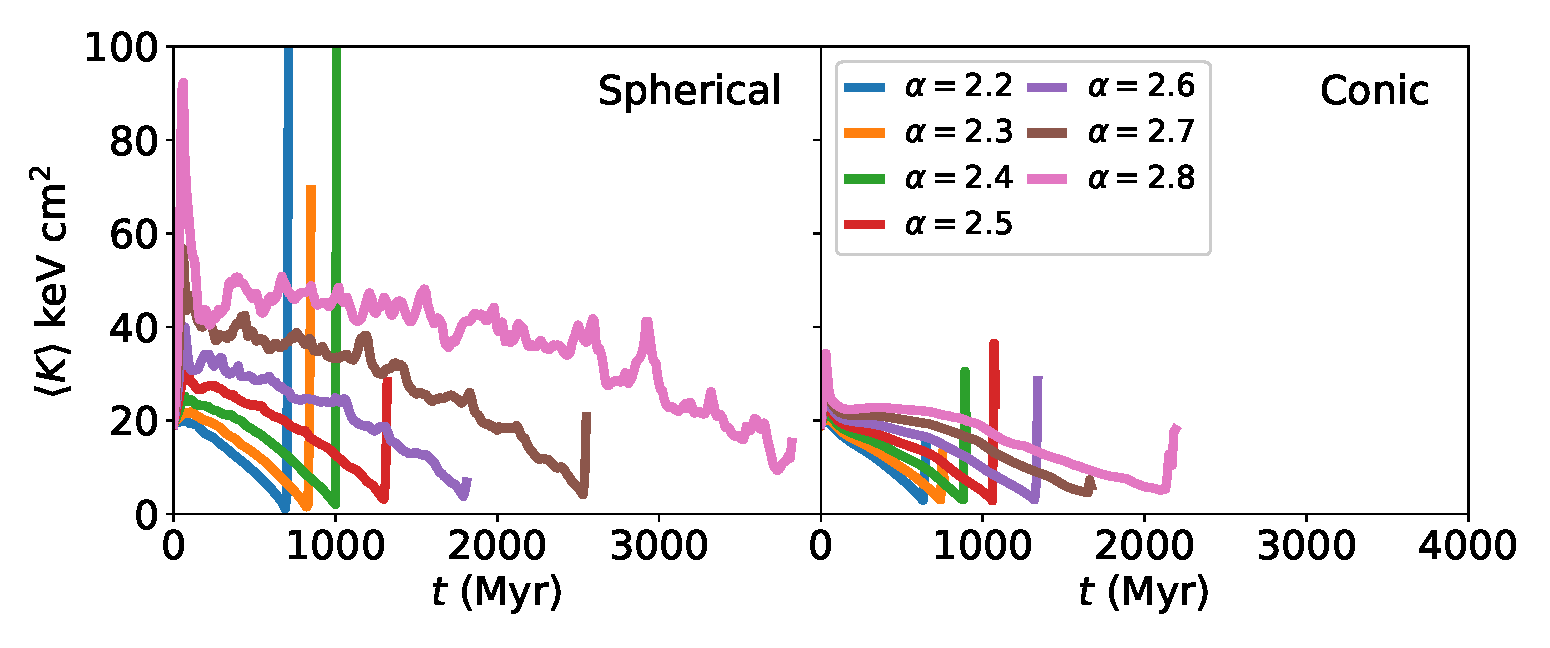
\includegraphics[width=1\linewidth]{figures/avgCoreEntropies.eps}
  \end{center}
  \caption{
    \label{fig:avgCoreEntropies}
    Mean entropy of the inner $10 \text{ kpc}$ proper as a function of time for
    simulations with radial exponents ranging from $\alpha=2.2$ to $\alpha=2.8$
    with spherical and conic feedback.  Mean entropy is calculated by the
    mass-weighted temperature and the volume-weighted density. To improve
    visibility, these are plotted up until $30 \text{ Myr}$ after the mean core
    entropy has increased by $60\%$ in a $10 \text{ Myr}$ span, or until the
    simulation has stopped. After this point, the entropy profile has diverged
    from what would be expected from observations. Simulations using values of
    $\alpha$ between those shown here were also run, although all exhibited the
    same core entropy decay with higher values of $\alpha$ decaying slower and
    conic feedback collapsing faster.
  }
\end{figure}

The purely thermal feedback failed to self regulate nor preserve thermal
stability. For all choices of $\alpha$ with either spherical or conic feedback,
the mean entropy of the inner $10 \text{ kpc}$ core fell over time, eventually
leading to a cooling driven collapse (fig. \ref{fig:avgCoreEntropies}.) Each
simulation formed a cold clump of gas around the core of the cluster (fig.
\ref{fig:phasePlots}) which began run away cooling and a spike in AGN activity
to match the cooling. Most simulations halted due
to hydrodynamics errors during this spike in feedback but a random selection of
simulations managed to evolve through the collapse. However, these simulations
had raised entropy profiles post-collapse which do not match observed entropy
profiles of CC clusters.

\subsection{Formation of Cold Gas}
\label{sec:formation_of_cold_gas}

In all cases with purely thermal heating, a cold clump of gas eventually formed
near the center of the cluster. Fig. \ref{fig:phasePlots} includes entropy and
cooling rate versus radius phase plots of the clusters at $t=50 \text{ Myr}$
(an arbitrary time step,) when the cold phase gas first appears in the
simulation, and at the final step when the either the simulation has reached
$t=800 \text{ Myr}$ or the hydrodynamics solver has failed. The formation of
the cold clump begins with a spreading of the entropy distribution at the
radius where the median entropy 
%and ratio of cooling time to free fall time
is minimized. Although the initial entropy profile has an isentropic core, as
do observations, the centralized thermal feedback causes the core entropy to
peak, leading to a minimal entropy region outside the core. Due to higher
energy deposition and therefore entropy peaks in the centers of high $\alpha$
simulations, the cold gas first forms further from the core for higher
$\alpha$.

When the coldest gas in the distribution reaches a critical specific entropy of
around $10^{-1} \text{ keV} \text{ cm}^2$, the cooling rate accelerates. This
gas quickly condenses into the cold phase. As the entropy distribution of the
hot phase continues to dip, more gas condenses onto the cold clump in a run
away collapse. 

Although the heating rate from the AGN ramps up with the accelerated cooling
rate, it is unable to immediately warm up nor push out the cold gas. The AGN
feedback spikes with the growth of the clump, eventually causing the
hydrodynamics solver to crash in most cases.

\subsection{High vs. Low $\alpha$}
\label{sec:high_vs_low_alpha}

Some differences between simulations arose between simulations using low
$\alpha<2.5$ (more dispersed thermal deposition) and high $\alpha>2.5$ ( more
centralized thermal deposition.) The high $\alpha$ feedback raised core
entropies higher above the initial entropy compared to low $\alpha$ runs by
raising core temperatures and pushing out gas to lower electron densities (fig.
\ref{fig:phasePlots}), as expected.  The increased entropy in the core from
increased energy deposition delayed the cooling driven collapse for a longer
period of time. This was also an expected result. Looking at fig.
\ref{fig:avgCoreEntropies}, higher $\alpha$ delayed the collapse super-linearly
compared to lower $\alpha$. However, it should be noted that percent of the
total feedback energy deposited in the core does not scale linearly with
$\alpha$ but asymptotes exponentially as $\alpha \rightarrow 3$.  Towards the
limiting case as $\alpha \rightarrow 3$ the majority of the feedback will
constrained to a small $r < 5 \text{ kpc}$ core, similar to the thermal only
feedback case from \cite{meece_triggering_2017}.
%, although the heating is triggered by the total cooling and not cold gas.

\begin{comment}
Additionally, by pushing more gas out of the core the cold clump that precedes
collapse forms outside of $r=1 \text{ kpc}$ in high $\alpha$ runs while the
cold clump forms in the center of the cluster in low $\alpha$ runs. However,
this distinct separation of where the cold clump forms may be due to high
$\alpha$ runs reaching the density floor of the simulation in their centers.
%With effectively no gas in the center at the density floor, a cold clump as
%the center can't be modeled
\end{comment}

\subsection{Mean Core Entropy} 
\label{sec:mean_core_entropy}

The mean core entropy in all simulations, both with spherical and conic
feedback, slowly fell until the formation of the cold clump in all simulations,
as is seen in fig.  \ref{fig:avgCoreEntropies}. At the formation of the cold
clump as the total cooling in the cluster spiked, the AGN activity also spiked,
causing the mean core entropy to also spike to unphysically high entropies.

High values of $\alpha$, or more centrally peaked feedback, maintained a higher
core entropy for a longer period of time. Initially the simulation is somewhat
stable, however cooling gas on the outskirts of the core lowers the mean core
entropy of the inner $10 \text{ kpc}$ (see fig. \ref{fig:phasePlots}.)  The
conic feedback was less efficient at maintaining core entropy. In all cases,
the conic feedback led to a quicker collapse. No quasi-stability was shown for
high values of $\alpha$ with conic feedback.

\begin{comment}
\FG{Make a footnote? Include in each plot?} Most plots in this section are
taken at $t = 500 \text{ Myr}$, an arbitrary time step after the initial
settling of the cluster and before collapse which demonstrates the approximate
structure of each simulation. Before $t=500 \text{ Myr}$ the higher $\alpha$
runs have not settled from the initial burst AGN activity while later than
$t=500 \text{ Myr}$ the lower $\alpha$ simulations have already collapsed. The
two $\alpha$ values $2.2$ and $2.8$ are used as the most extreme values of
$\alpha$ simulated that evolved to $t= 500 \text{ Myr}$ without collapsing.
\end{comment}

\begin{figure*}
	\begin{center}
    \includegraphics[width=1\linewidth]{figures/radius_entropy_profiles.eps}
		\includegraphics[width=1\linewidth]{figures/radius_cooling_rate_profiles.eps}
	\end{center}
	\caption{
    \label{fig:phasePlots}
    Phase plots of entropy and cooling rate versus radius of simulations with
    spherical and conic AGN heating with radial exponents $\alpha=2.2$ and
    $\alpha=2.8$ as labeled, with the initial and current median entropy or
    cooling rate versus radius in dashed blue and solid black respectively. The
    total heating rate in a shell versus radius is superimposed on the cooling
    rate in solid red, which is scaled in the simulation to match in total
    cooling rate.  The upper plots are at $t= 500 \text{ Myr}$ and the lower
    plots are at the final time step of the simulation.
    %\FG{Should I include the final step? Maybe more a time sequence through
    %collapse of one simulation? Combine r axes. Also, maybe a radial profile
    %of cold gas to see where it forms}
  }
\end{figure*}

\subsection{Phase Plots}
\label{sec:phase_plots}

Fig. \ref{fig:phasePlots} shows phase plots of entropy and the cooling rate
versus radius. As expected, at $t= 500 \text{ Myr}$ the higher $\alpha=2.8$ run
has a higher core entropy than $\alpha=2.2$ since more energy is deposited in
the center. The median entropy profile still follows the initial median but
there is more high entropy gas near the core. Both the spherical and conic
$\alpha=2.2$ evolved past their collapse but are left with core entropy
profiles too high to match observations. The $\alpha=2.8$ simulations formed
cold gas near their cores as they collapsed before hydrodynamic errors stopped
the simulations.  The heating rate is also plotted with the median cooling in
the cooling rate phase diagram. For certain values of $\alpha$, heating exceeds
cooling in the inner core and outer radii but not in the intermediate range
where the entropy profile changes from a flat line to a power law. 
However, this criterion was not
enough to produce thermally stable clusters.
%\FG{This would make more sense with volume averaged cooling rate instead of
%the median - that's what should be directly compared.} 


\begin{comment}
\begin{figure*}
	\begin{center}
		\includegraphics[width=0.49\linewidth]{figures/entropy_slices}
		\includegraphics[width=0.49\linewidth]{figures/density_slices}
		\includegraphics[width=0.49\linewidth]{figures/temperature_slices}
		\includegraphics[width=0.49\linewidth]{figures/cooling_rate_slices}
	\end{center}
	\caption{
    \label{fig:slices}
    Slices of entropy, density, temperature, and cooling rate through the
    origin of simulations with spherical and conic AGN heating with radial
    exponents $\alpha=2.2$ and $\alpha=2.8$ as labeled. All data is taken at
    $t= 500 \text{ Myr}$. \FG{Are these figures worth including? Combine x and y axes?}}
\end{figure*}

Fig. \ref{fig:slices} shows slices through the origin of the entropy, density,
temperature, and cooling rate of simulations with spherical and conic heating
with $\alpha=2.2$ and $\alpha=2.8$, two more extreme values of $\alpha$. In
both high $\alpha$ simulations, the core entropy and temperature are raised
while the core density and cooling rate is lower. In the conic simulations, the
jet structure is more apparent in high $\alpha$ cases. The jet is also more
collimated than would be expected for the $\cos^2 \theta$ dependence used,
although this may be due to the small radius where the majority of the energy
is deposited in the high $\alpha$ case.
\end{comment}

\begin{comment}
\begin{figure}
  \caption{Cold gas fraction as a function of time}
\end{figure}
\end{comment}

\section{Discussion}
\label{sec:discussion}

\subsection{Thermal Stability}
\label{sec:thermal_stability}

In all simulations explored here, the purely thermal heating was unable to
prevent a run-away cooling collapse. The distributions of AGN heating did not
prevent the formation and growth of cold clumps nor push them out of the core
without dumping unphysically high amounts of energy. These shortcomings of a
thermal only AGN heating model are in line with simulation work from
\citep{gaspari_agn_2011,meece_triggering_2017}.

High values of $\alpha$, or more centrally peaked feedback, did prevent the
cooling collapse for a longer period. 

Comparing to previous work in \citep{gaspari_agn_2011,meece_triggering_2017},
this current work reaffirms the necessity of kinetic outflows, or at least some
mechanism beyond thermal heating, to push cold clumps of gas out of the
isentropic zone and into the power-law entropy zone where their condensation
may be suppressed.

The contrived direct coupling of the AGN feedback to the total cooling rate of
the cluster also led to simulation issues when compared to Bondi accretion and
cold gas accretion models used in other works \cite{meece_triggering_2017}. As
the gas collapsed into the cool phase, the cooling rate spiked, leading the
heating rate to reach unphysically high levels. If the hydrodynamics solver did
not fail through the collapse, the high heating rate pushed the isentropic
region of the cluster to much higher entropy levels than the initial
conditions. Although Bondi accretion and cold gas accretion models increase
feedback with the formation of cold gas and higher densities, they do not raise
the heating rate to as high levels as seen here.

Higher $\alpha$, corresponding to more energy input at the cluster core,
predictably raised core entropy. Lower $\alpha$ left a flat entropy
profiles closer to the initial conditions.  The higher $\alpha$
simulations push out enough gas from the core to decrease x-ray
brightness. 

\subsection{Comparison to Observation}
\label{sec:comparison_to_observation}

Although the simulations did not achieve thermal stability, we can still
compare some results to observations, particularly entropy and surface
brightness profiles from the ACCEPT dataset \cite{cavagnolo_intracluster_2009}.

\begin{figure}
	\begin{center}
		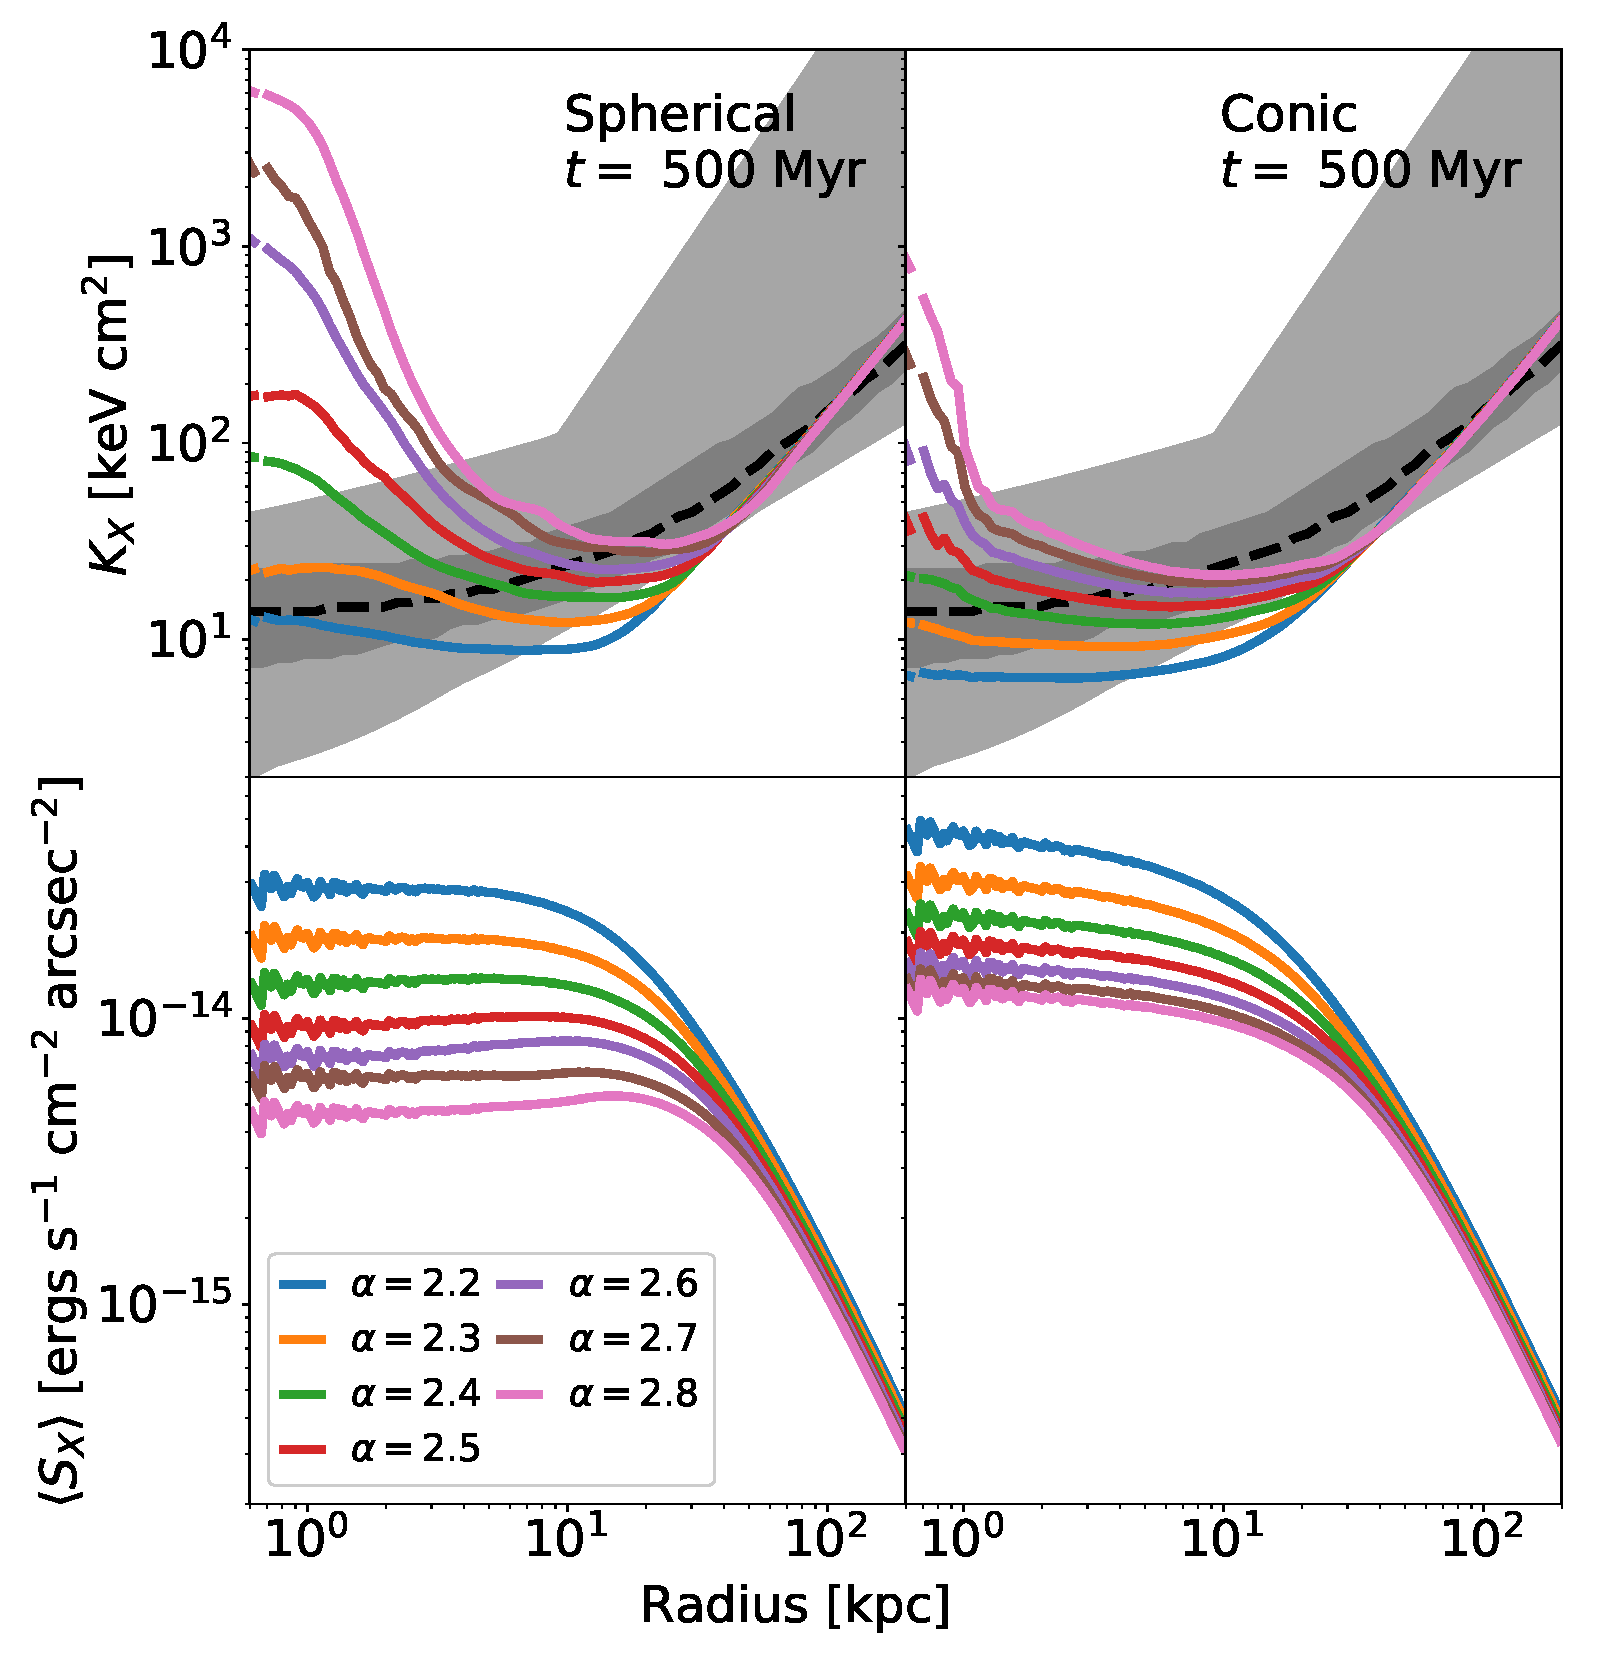
\includegraphics[width=1\linewidth]{figures/allVradius.eps}
	\end{center}
	\caption{
    \label{fig:allVradius}
    \textbf{Top:} Mean entropy as a function of spherical radius from
    several representative simulations using different radial exponents
    $\alpha$ for heating with spherical feedback (left) and conic feedback
    (right.) Mean entropy is calculated by the mass-weighted temperature and the
    volume-weighted density. Entropy profiles
    of CC clusters from the ACCEPT dataset are included in the shaded regions,
    with the dashed line denoting the median, the darker region denoting the
    $68\%$ confidence interval, and the lighter region denoting the extent of
    the CC clusters in the dataset. Entropy profiles from the ACCEPT dataset
    were generated from the $K = K_0 + K_{100} \left ( r/100 \text{ kpc}
    \right )^{\alpha_k}$ fits from the dataset. Only CC clusters defined by $K_0
    < 30 \text{ keV cm}^2$ from ACCEPT are shown, giving 141 clusters.
    \textbf{Bottom:}	Mean simulated X-ray surface brightness in the $0.5 - 2.0
    \text{keV}$ band of cores of radii $R = 2^0 - 2^4$ proper kpc from as a
    function of $\alpha$ for heating with spherical feedback (left) and conic
    feedback (right.) 
    \textbf{Bottom:}Mean simulated X-ray surface brightness in the $0.5 -2.0
    \text{ keV}$ band as a function of observing radius from several
    representative simulations using different radial exponents $\alpha$ for
    heating with spherical feedback (left) and conic feedback (right.) All data
    is taken at $t= 500 \text{ Myr}$.
  }
    %\FG{Add density? Add text annotations?
    %Combine with fig. \ref{fig:allValpha}? Combine spherical and conic onto one
    %plot?
\end{figure}

In fig. \ref{fig:allVradius}, we compare the entropy profiles of several
representative simulations to entropy profiles from fits from the ACCEPT
dataset, as well show surface brightness profiles. Entropy profiles from the
simulations were calculated using the mass-weighted temperature and the
volume-weighted density, following \citep{}. Confidence intervals of entropy
profiles from the ACCEPT data were generated using the $K = K_0 + K_{100} \left
( r/100 \text{ kpc} \right )^{\alpha_k}$ fits. Only CC clusters are
considered, defined here as having $K_0 < 30 \text{ keV cm}^2$. Simulation data
was examined at $t = 500 \text{ Myr}$, although it should be noted that this is
an arbitrary time step. As the higher $\alpha$ simulations drop in core
entropy, their entropy profiles will look more similar to the lower $\alpha$
simulations at earlier time steps. The initial conditions chosen also fall
outside the ACCEPT dataset, which may affect comparisons.

The simulation data with purely thermal feedback shows peaked entropy profiles
towards the core, inherently in contrast to the power-law profiles generated
from the ACCEPT dataset. The difference is largest for high $\alpha$, given
their centralized feedback. These may be ruled out as unphysical for
simplified models of purely thermal AGN feedback.  The lower $\alpha$
simulations may have more acceptable profiles, although even with a small peak
in entropy they quickly collapse.

The x-ray surface brightness profiles experience less variation with changes in
$\alpha$. A high $\alpha$ pushes more mass out of the core, leading to less
matter to radiate which lowers the surface brightness.

\begin{figure}
	\begin{center}
		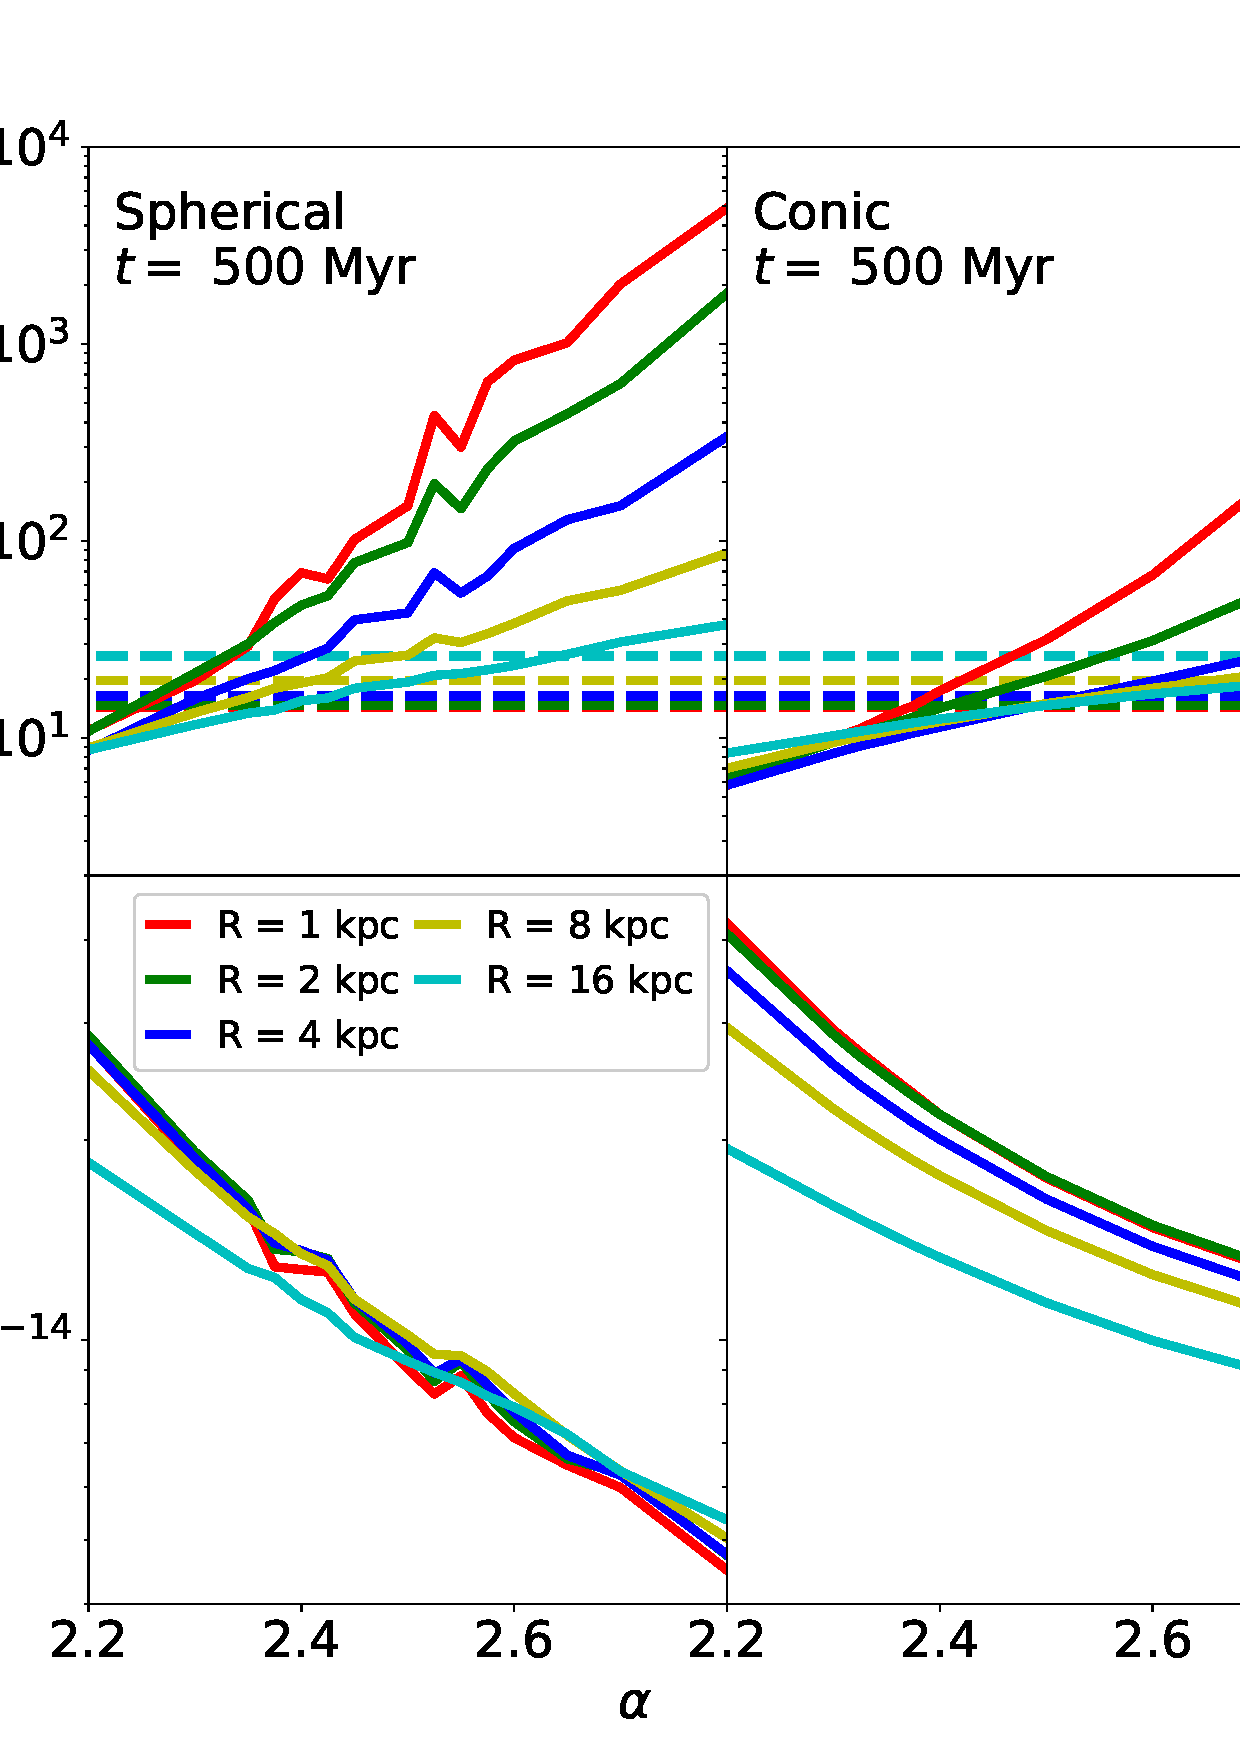
\includegraphics[width=1\linewidth]{figures/allValpha.pdf}
	\end{center}
	\caption{
    \label{fig:allValpha}
    \textbf{Top:}  Mean cluster core entropy calculated within impact
    parameters ranging from $R = 2^0 - 2^4$ proper kpc as a function of
    $\alpha$ for heating with spherical feedback (left) and conic feedback
    (right.) Mean entropy from simulation results is calculated by the
    mass-weighted temperature and the volume-weighted density. Entropy profiles
    of CC clusters from the ACCEPT dataset are included in the shaded regions,
    with the dashed lines denoting the mean core entropy within various radii
    produced from the median entropy profile. Entropy profiles from the ACCEPT
    dataset were generated from the $K = K_0 + K_{100} \left ( r/100 \text{
      kpc} \right)^{\alpha_k}$ fits from the dataset. Only CC clusters defined
    by $K_0 < 30 \text{ keV cm}^2$ from ACCEPT are shown, giving 141 clusters.
    \textbf{Bottom:}	Mean simulated X-ray surface brightness in the $0.5 - 2.0
    \text{keV}$ band of cores of radii $R = 2^0 - 2^4$ proper kpc from as a
    function of $\alpha$ for heating with spherical feedback (left) and conic
    feedback (right.) All data is take at $t= 500 \text{ Myr}$.}
\end{figure}

Mean core entropies and surface brightness for different $\alpha$ within
different core sizes are shown in fig. \ref{fig:allValpha}, with more
comparisons to ACCEPT data. The mean core entropy increases with $\alpha$ while
the surface brightness decreases.  Due to the central entropy peak present in
all simulations at $t= 500 \text{ Myr}$ (expect for low $\alpha$ conic
simulations, which are beginning to collapse,) the mean core entropy increases
with smaller size cores, in contrast to the observed power-laws from ACCEPT
where the entropy flattens at the center. Ideally, the mean core entropies
should intersect the dashed lines indicated ACCEPT entropy medians at one value
$\alpha$ rather than all at wildly different values of $\alpha$. The central
entropy peak prevents this. 

\subsection{ Possible Conclusions}
\label{sec:possible_conclusions}

Due to the failure to produce even quasi-stable clusters with realistic entropy
profiles and the absence of a preferred time step in the cluster evolution
before the formation of the cold phase, comparisons to observation may not be
accurate. However, a few possible conclusions can be made. 

In the context of purely thermal AGN feedback, highly centrally concentrated
feedback (corresponding to high $\alpha > 2.5$ simulations) produce
unphysically high entropy cores. These may be ruled out from simplified AGN
feedback models.

When the heating rate was directly tied to the total cooling rate in the
cluster, the rapid cooling of gas into cold clumps caused the heating rate to
reach unphysically high levels. This is in contrast to simulations using Bondi
accretion and cold gas accretion such as in \cite{meece_triggering_2017}, where
the AGN feedback still increases with the formation of cold gas but can be
tuned to stay within physically reasonable values.

The basic power-law AGN thermal heating considered here are unable to maintain
thermal stability of the cluster. In cases, when a cold clump of gas forms, the
simulation is unable to disrupt the clump without injecting unphysically high
amounts of energy. The thermal heating in these simulations was unable to
replace kinetic outflows from AGN jets such as in
\citep{meece_triggering_2017}. However, a purely thermal model may still exist,
although with more parameters and constraints, which can mimic observed CC
clusters.


\section{Summary}
\label{sec:summary}

We have presented simulation results for simplified models of AGN feedback
using purely thermal feedback following a radial power law, $\dot e \propto
r^{-\alpha}$ dependence, where the total feedback is scaled to the total
cooling within the clusters. All cases of this setup failed to maintain thermal
stability with observationally reasonable entropy profiles (see figs.
\ref{fig:avgCoreEntropies},\ref{fig:phasePlots}.) The purely thermal feedback was unable
to suppress the formation of a large cold clump of gas while the increased
cooling rate through this process raised the heating rate to very high levels.

We also compared entropy profiles from these results to observational data from
the ACCEPT dataset. Our simulations exhibited small to large central peaks in
entropy which differ from the power-law entropy profiles from ACCEPT. The
entropy peaks were more pronounced for higher values of $\alpha$ due to the
more centralized feedback. Simplified AGN models with centralized thermal
heating are unlikely to produce realistic entropy profiles.

A few possible conclusions can be made from this work. Highly centralized
feedback produces unreasonable high entropy profiles compared to observations.
These can a eliminated from simplified models of AGN feedback.  An AGN heating
rate directly tied cooling rate led to a sharp jump in feedback as cold gas
formed in the simulation. This differs from previous simulations approximating
feedback rates using Bondi and cold gas accretion models, which can temper the
feedback.  No configuration of purely thermal feedback explored here achieved
thermal stability nor prevented a run away collapse into a cold clump, in
contrast to previous simulations included kinetic jets. However, a purely
thermal model for AGN feedback may still exist that can produce realistic CC
clusters, although more constraints on the heating will be necessary.

\begin{comment}
Although this is a very simplified model of cluster feedback, it can be used to
constrain the broad properties of AGN feedback -- in particular, the radial
dependence of its heat deposition -- using X-ray observations.  In the near
future, we will make direct comparisons to Chandra X-ray data of entropy and
surface brightness profiles  using the ACCEPT survey
\cite{cavagnolo_intracluster_2009} and its successors.
\end{comment}

\begin{comment}


  Ideally, what should happen? (it's not reproducing Greg's sims)
  Multiphase region in isentropic region, cold gas clumps condense out of
  muliphase region, they are pushed out to power-law zone in outflows/bounacy,
  they disapate/condensing suppressed by bounacy in power-law zone.

  What we see:
  Our refinement isn't high enough to get cold gas condensing before it
  collapses?
  As soon as a cold gas clump condenses, it collapses. (As it should? it's going to self-regulate)

  But as soon as the cold gas clump condenses, the cooling rate skyrockets, and
  so does the heating rate This is unphysical

  Greg's simulations also formed cold clumps, including the kinetic jet ones.
  It's just that with cold mass accretion, the heating rate was limited. With
  ours it exploded, leading to the hydro errors.

  If our evolved through the collapses, would they be reasonable/acceptable?
  Alpha 2.4's entropy profile doesn't look too bad - are they observationally reasonable?.


  The entropy/surface brightness plot vs. radius/alpha is misleading, since
  there is no preferred time step except the initial time step and the
  formation of the cold clump. I could find separate time steps for the higher
  alpha=2.8 runs that would have entropy profiles that roughly match the lower
  alphas ~2.2 at earlier timesteps.

  Resolutions:
    Evolve current sims through collapse and compare to observations/Meece data
      -to see if these behave like Meece's work (and like the theory?)

    Evolve with direct feedback+cold gas accretion

    Evolve with PPM (just because)
    Evolve with higher AMR (just because)

\end{comment}

\acknowledgments
\section{Acknowledgments}
\label{sec:acknowledgments}
This project has been supported by NASA through Astrophysics Theory Program
grant \#NNX15AP39G and Hubble Theory Grant HST-AR-13261.01-A, and by the
NSF through grant AST-1514700.  The simulations were run on the NASA
Pleiades supercomputer through allocation SMD-16-7720.  \texttt{Enzo} and
\texttt{yt} are developed by a large number of independent researchers from
numerous institutions around the world. Their commitment to open science
has helped make this work possible.

%\input{apj-bib}
\bibliographystyle{apj}

\bibliography{apj-jour,AGNThermal2018}

\end{document}
